\begin{enumerate}[label=\thesection.\arabic*,ref=\thesection.\theenumi]
\item You are riding in an automobile of mass 3000 kg. Assuming that you are examining the oscillation characteristics of its suspension system. The suspension sags 15 cm when the entire automobile is placed on it. Also, the amplitude of oscillation decreases by 50\% during one complete oscillation. Estimate the values of
\begin{enumerate}[label=(\alph*)]
    \item The spring constant \( K \)
    \item The damping constant \( b \) for the spring and shock absorber system of one wheel, assuming that each wheel supports 750 kg.
\end{enumerate}
\solution
\iffalse
\let\negmedspace\undefined
\let\negthickspace\undefined
\documentclass[journal,12pt,twocolumn]{IEEEtran}
\usepackage{cite}
\usepackage{amsmath,amssymb,amsfonts,amsthm}
\usepackage{algorithmic}
\usepackage{graphicx}
\usepackage{textcomp}
\usepackage{xcolor}
\usepackage{txfonts}
\usepackage{listings}
\usepackage{enumitem}
\usepackage{mathtools}
\usepackage{gensymb}
\usepackage{comment}
\usepackage[breaklinks=true]{hyperref}
\usepackage{tkz-euclide}
\usepackage{listings}
\usepackage{gvv}
\def\inputGnumericTable{}
\usepackage[latin1]{inputenc}
\usepackage{color}
\usepackage{array}
\usepackage{longtable}
\usepackage{calc}
\usepackage{multirow}
\usepackage{hhline}
\usepackage{ifthen}
\usepackage{lscape}
\usepackage{float}

\newtheorem{theorem}{Theorem}[section]
\newtheorem{problem}{Problem}
\newtheorem{proposition}{Proposition}[section]
\newtheorem{lemma}{Lemma}[section]
\newtheorem{corollary}[theorem]{Corollary}
\newtheorem{example}{Example}[section]
\newtheorem{definition}[problem]{Definition}
\newcommand{\BEQA}{\begin{eqnarray}}
\newcommand{\EEQA}{\end{eqnarray}}
\newcommand{\define}{\stackrel{\triangle}{=}}
\theoremstyle{remark}
\newtheorem{rem}{Remark}
\begin{document}

\bibliographystyle{IEEEtran}
\vspace{3cm}

\title{ANALOG}
\author{EE23BTECH11006 - Ameen Aazam$^{*}$% <-this % stops a space
}
\maketitle
\newpage
\bigskip

\renewcommand{\thefigure}{\theenumi}
\renewcommand{\thetable}{\theenumi}

\vspace{3cm}
\textbf{Question :}
You are riding in an automobile of mass 3000 kg. Assuming that you are examining the oscillation characteristics of its suspension system. The suspension sags 15 cm when the entire automobile is placed on it. Also, the amplitude of oscillation decreases by 50\% during one complete oscillation. Estimate the values of
\begin{enumerate}[label=(\alph*)]
    \item The spring constant \( K \)
    \item The damping constant \( b \) for the spring and shock absorber system of one wheel, assuming that each wheel supports 750 kg.
\end{enumerate}
\begin{enumerate}
	\item{\texbf{Solution :}}
\end{enumerate}
\fi
    \textbf{Parameters:}
    \begin{table}[htbp]
        \centering
        \begin{tabular}{|l|l|l|}
\hline
\textbf{Parameter} & \textbf{Value(SI)} & \textbf{Description} \\ \hline
$x_{0}$ & 0.15 & Initial spring compression \\ \hline
$m$          & 750 & Mass              \\ \hline
$g$          & 9.8 & Gravitational acc \\ \hline
$k$          & $mg/x_{0}$ & Spring constant   \\ \hline
$b$          &  & Damping constant  \\ \hline
\end{tabular}

        \vspace{5pt}
        \caption{Input Parameters}
        \label{tab:Table 1}
    \end{table}
    \begin{table}[htbp]
        \centering
        \begin{tabular}{|l|l|l|}
\hline
\textbf{Parameter} & \textbf{Value(SI)} & \textbf{Description} \\ \hline
$x$          &  & Spring Extension \\ \hline
$F_1$ & $kx$ & Spring Force \\ \hline
$F_2$ & $b\frac{dx}{dt}$ & Damping Force \\ \hline
$s$ & & Complex Frequency \\ \hline
$s_1, s_2$          &  & Values of s \\ \hline
\end{tabular}

        \vspace{5pt}
        \caption{Intermediate Parameters}
        \label{tab:Table 2}
    \end{table}
    
    \vspace{15pt}
    


    Initially the automobile is in rest, so we can use,
    \begin{align}
        &mg = kx_0 \label{eq:1}\\
        \implies &k=\frac{mg}{x_0} \label{eq:2}
    \end{align}

    \begin{figure}[h]
        \centering
        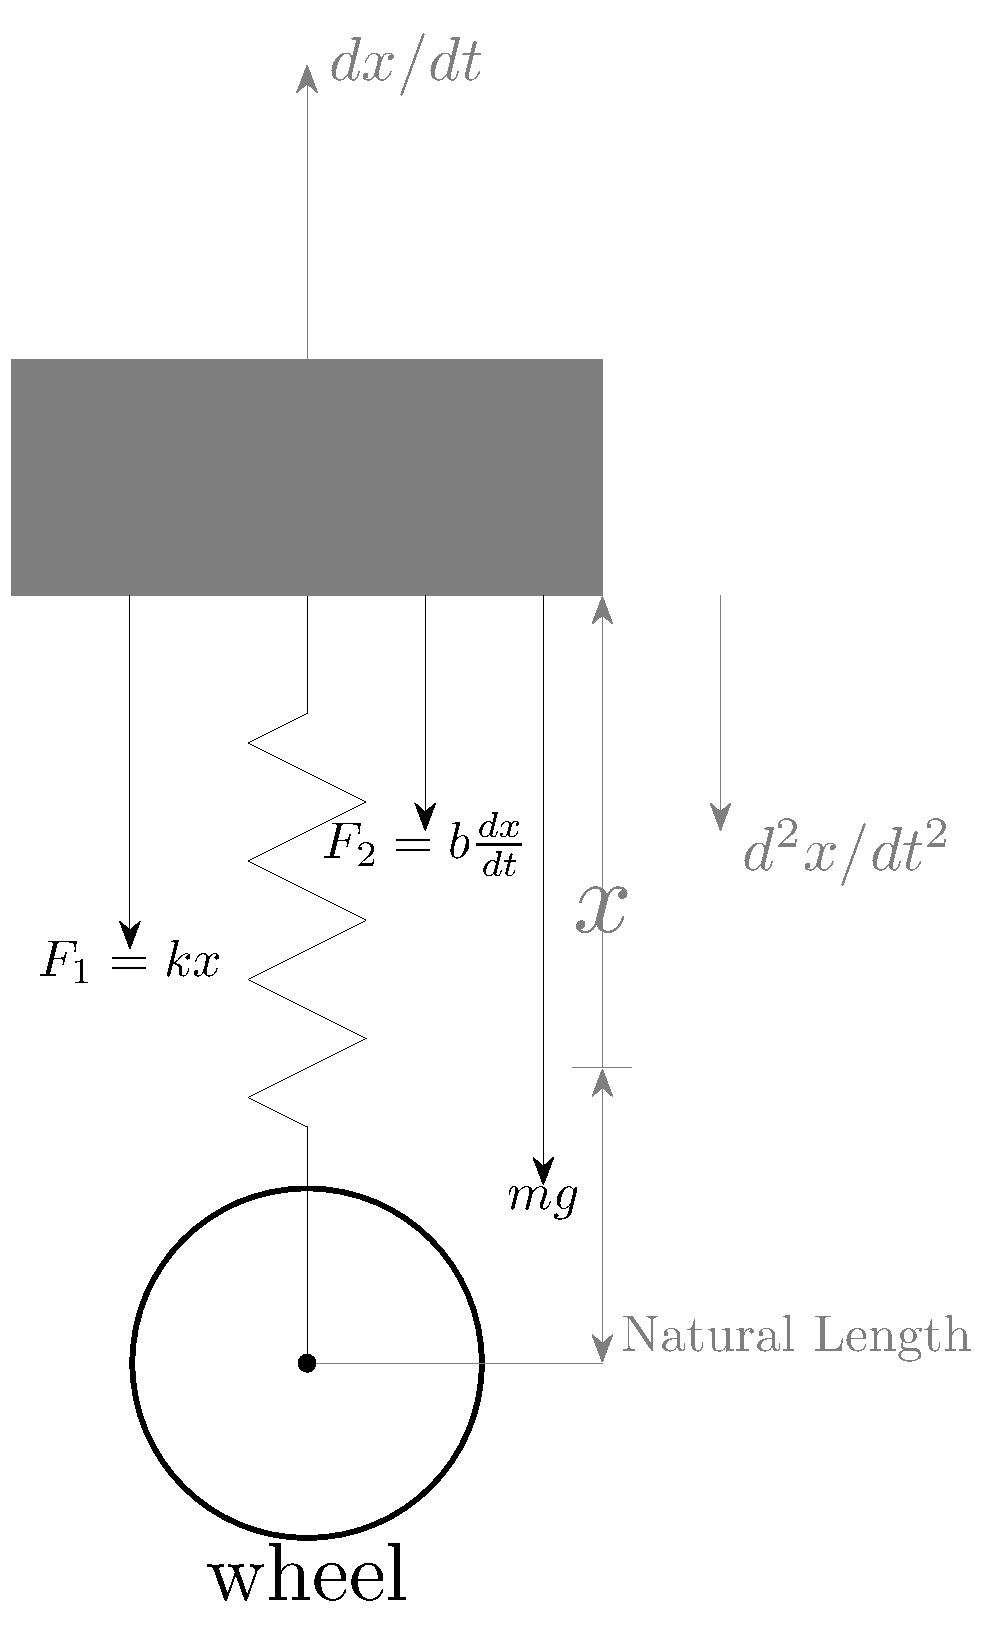
\includegraphics[width=0.6\columnwidth]{ncert-physics/11/14/figs/11_14_21_fbd.pdf}
        \caption{FBD of the damped oscillation system}
        \label{fig:Fig-1}
    \end{figure}

    Now, as the oscillation begins, from the \figref{fig:Fig-1} we net force on the mass as,
    \begin{align}
        &F=F_{1}+F_{2}+mgu(t) \label{eq:3}\\
        \implies &-m\frac{d^2x(t)}{dt^2}=kx(t)+b\frac{dx(t)}{dt}+mgu(t) \label{eq:4}\\
        \implies &\frac{d^2x(t)}{dt^2}+\brak{\frac{b}{m}}\frac{dx(t)}{dt}+\brak{\frac{k}{m}}x(t)=-gu(t) \label{eq:5}
    \end{align}

    Now, taking the Laplace transform on both sides,
    \begin{align}
        &s^2X(s)+\frac{b}{m}sX(s)+\frac{k}{m}X(s)=-\frac{g}{s} \label{eq:6}\\
        \implies &X(s)=-\frac{g}{s\brak{s^2+\frac{b}{m}s+\frac{k}{m}}} \label{eq:7}\\
        \implies &X(s)=-\frac{g}{s(s-s_1)(s-s_2)} \label{eq:8}
    \end{align}
    Where
    \begin{align}
        &s_1=-\frac{b}{2m}+\sqrt{\brak{\frac{b}{2m}}^2-\frac{k}{m}} \label{eq:9}\\
        &s_2=-\frac{b}{2m}-\sqrt{\brak{\frac{b}{2m}}^2-\frac{k}{m}} \label{eq:10}
    \end{align}
    From \eqref{eq:8} we get,
    \begin{align}
        \begin{split}
            \implies &X(s)=\frac{g}{(s_1-s_2)}\sbrak{\frac{1}{s_2(s-s_2)}-\frac{1}{s_1(s-s_1)}} \\
            &+\frac{g}{s_1s_2}\brak{\frac{1}{s}} \label{eq:11}
        \end{split}
    \end{align}
    Now again taking the inverse Laplace transform we have,
    \begin{align}
        &x(t)=\frac{g}{s_1s_2}u(t)+\frac{g}{(s_1-s_2)}\sbrak{\frac{1}{s_2}e^{s_2t}-\frac{1}{s_1}e^{s_1t}}u(t)\label{eq:12}
    \end{align}
    \begin{align}
    \begin{split}
    \implies &x(t) =\sqrt{\brak{\frac{mg}{k}}^2 + \brak{\frac{gb}{2mk}}^2}e^{-bt/2m}u(t) \\
            &\sin{\brak{\sqrt{\frac{k}{m} - \brak{\frac{b}{2m}}^2}t + \tan^{-1}\brak{\frac{2mg\sqrt{\frac{k}{m} - \brak{\frac{b}{2m}}^2}}{gb}}}} \\
            &+ \frac{mg}{k}
        u(t) \label{eq:13}
\end{split}
\end{align}
    (Substituting the values of $s_1$ and $s_2$ from \eqref{eq:9} and \eqref{eq:10})

    From \eqref{eq:13} we have the amplitude after one time period $T$,
    \begin{align}
        \begin{split}
            &\frac{1}{2}\sqrt{\brak{\frac{mg}{k}}^2+\brak{\frac{gb}{2mk}}^2}= \\
            &\sqrt{\brak{\frac{mg}{k}}^2+\brak{\frac{gb}{2mk}}^2}e^{-bT/2m} \label{eq:14}
        \end{split}
    \end{align}
    \begin{align}
        \implies &e^{\pi b/\sqrt{mk}}=2 \label{eq:15}\\
        \implies &b=\frac{\sqrt{mk}\ln{2}}{\pi} \label{eq:16}
    \end{align}
    \begin{figure}[h]
        \centering
        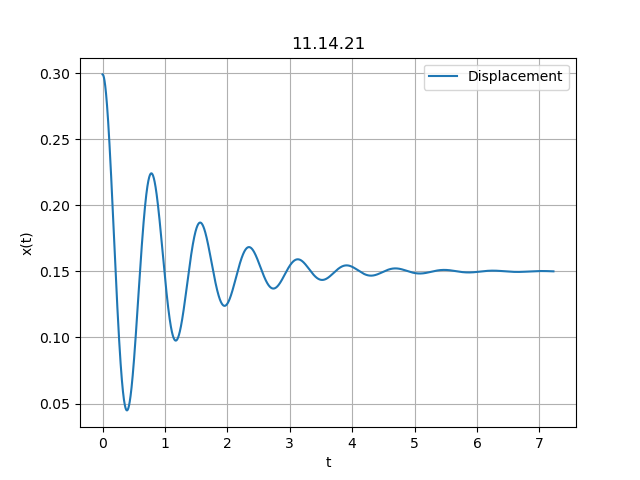
\includegraphics[width=0.8\columnwidth]{ncert-physics/11/14/figs/11.14.21_plot.png}
        \caption{Displacement Vs. Time Graph}
        \label{fig:Fig-2}
    \end{figure}

%\end{document}

\pagebreak
\item A mass attached to a spring is free to oscillate, with angular velocity $\omega$, in a horizontal
plane without friction or damping. It is pulled to a distance $x_0$
 and pushed towards
the centre with a velocity $v_0$
 at time t = 0. Determine the amplitude of the resulting
oscillations in terms of the parameters $\omega{}$, $x_0$,
 and $v_0$
. [Hint : Start with the equation
$x = a \cos\brak{\omega{t}+\theta{}}$ and note that the initial velocity is negative.]
\solution
\pagebreak
\end{enumerate}
